\chapter{Topology dataset analysis}
\label{chapter:dataset}

\section*{Introduction}

In this chapter we provide a brief description of the dataset used in the experimental evaluation of this thesis.

We use four groups of topologies: the RocketFuel topologies \cite{rocketfuel} which contains 6 topologies, the topologies from the
topology Zoo \cite{internetzoo-jsac11} which consists of 520 topologies of and 3 private ISP topologies and a topology of the
OVH-Europe network \cite{OVH}. The later topology is important because if contains a lot of link bundles (parallel links) which is a 
property that is often ignored in the algorithmic community. A lot of graph algorithms assume that the graphs are simple
and therefore there are not a lot of empirical results over these kinds of topologies.

These topologies were cleaned so that each of them contains only one strongly connected component, meaning
that there is at least one path between each pair of nodes in each topology. This is a simple cleaning step that is necessary because
it does not make sense to have a network topology where some nodes cannot communicate with each other.

\section{Topology sizes}

Tables \ref{fig:rf_sizes}, \ref{fig:real_sizes} and \ref{fig:zoo_sizes} show the sizes of the topologies in each
of the groups considered in this thesis. For the \texttt{zoo} group we only show the largest topologies since on one
hand those are the most relevant for our evaluation and the group contains too many topologies allows for a complete
listing.

In table \ref{fig:sizes} we show the
minimum and maximum sizes of the topologies in our dataset and table \ref{fig:group_sizes} shows the percentage of topologies whose
number nodes lies in different sizes. This shows that we tackle a wide range
of topologies of realistic sizes. 

%\begin{figure}
%\begin{center}
%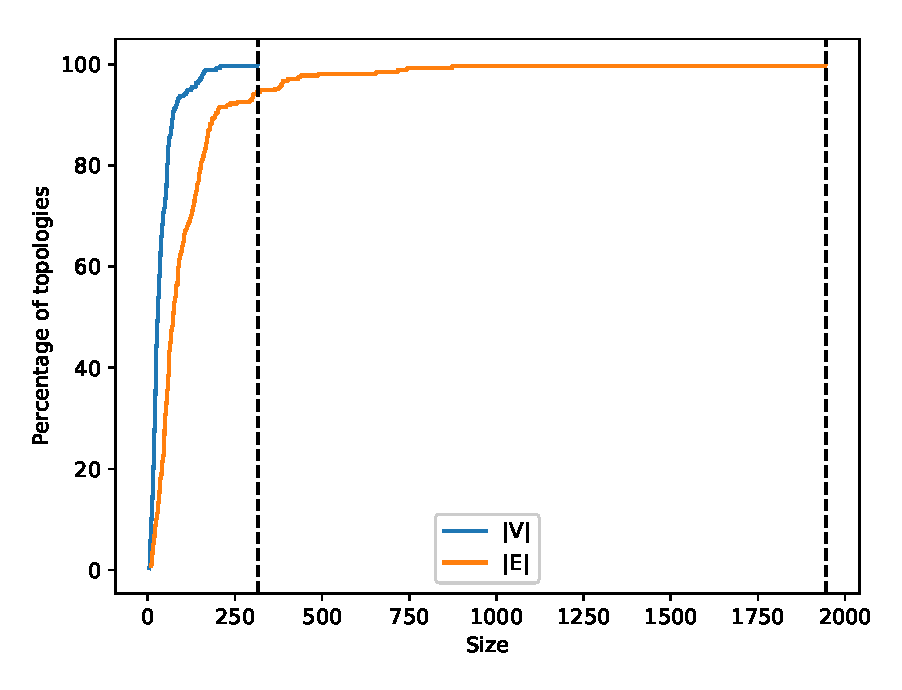
\includegraphics[width=.85\columnwidth]{./Network-lib/data/plot/topology_sizes.eps}
%\end{center}
%\caption{Distribution of the topology sizes.}
%\label{fig:sizes}
%\end{figure}

\begin{figure}
\begin{center}
\begin{tabular}{lrr}
\toprule
Topology name & $|V(G)|$ & $|E(G)|$\\
\midrule
AS 1221 & 104 & 302  \\
AS 1239 & 315 & 1944 \\
AS 1755 & 87 & 322   \\
AS 3257 & 161 & 656  \\
AS 3967 & 79 & 294   \\
AS 6461 & 138 & 744  \\
\bottomrule
\end{tabular}
\end{center}
\caption{Topology sizes in the \texttt{rf} group.}
\label{fig:rf_sizes}
\end{figure}

\begin{figure}
\begin{center}
\begin{tabular}{lrr}
\toprule
Topology name & $|V(G)|$ & $|E(G)|$\\
\midrule
ISP 1 & $\approx 150$ & $\approx 700$ \\
ISP 2 & $\approx 220$ & $\approx 800$ \\
ISP 3 & $\approx 170$ & $\approx 440$ \\
OVH   & 57 & 402 \\
\bottomrule
\end{tabular}
\end{center}
\caption{Topology sizes in the \texttt{real} group and \texttt{ovh}.}
\label{fig:real_sizes}
\end{figure}


\begin{figure}
\begin{center}
\begin{tabular}{lrr}
\toprule
Topology name & $|V(G)|$ & $|E(G)|$\\
\midrule
ITZ Cogentco  & 197 & 490 \\
ITZ Colt      & 153 & 382 \\
ITZ Deltacom  & 113 & 366 \\
ITZ Dia       & 138 & 302 \\
ITZ GtsCe     & 149 & 386 \\
ITZ Interoute & 110 & 312 \\
ITZ Ion       & 125 & 300 \\
ITZ Tata      & 145 & 388 \\
ITZ UsCarrier & 158 & 378 \\
\bottomrule
\end{tabular}
\end{center}
\caption{Largest topologies in the \texttt{zoo} group.}
\label{fig:zoo_sizes}
\end{figure}

\begin{figure}
\begin{center}
\begin{tabular}{cccc}
\toprule
Min $|V(G)|$ & Max $|V(G)|$ & Min $|E(G)|$ & Max $|E(G)|$ \\
\midrule
4 & 315 & 8 & 1955 \\
\bottomrule
\end{tabular}
\end{center}
\caption{Minimum and maximum topology sizes.}
\label{fig:sizes}
\end{figure}

\begin{figure}
\begin{center}
\begin{tabular}{cccc}
\toprule
Small & Medium & Large & Huge \\
$[0, 20]$ & $]20, 50]$ & $]50, 100]$ & $> 100$ \\
\midrule
30\% & 43\% & 21\% & 6\% \\
\bottomrule
\end{tabular}
\end{center}
\caption{Number of topologies by group size.}
\label{fig:group_sizes}
\end{figure}

\section{ECMP and non shortest path links}

We mentioned in the introduction that segment routing supports two kinds of segments: node segments 
and adjacency segments. We will see that adjacency segments are more costly and thus we would like to avoid using them whenever possible. However,
will see later that adjacency segments in segment routing can we necessary to implement paths that belong to ECMP components or that traverse
links that do not belong to any IGP shortest path. For that reason we analyzed the amount of ECMP component that exist in out dataset as well
as the amount of edges that do not belong to any shortest path. These values will give an estimation of how important supporting adjacency segments
is. Figure \ref{fig:ECMPcount} shows the percentage of links that do not belong to any shortest path as well as the percentage of pairs
of nodes with ECMP between them. We can see that, as expected, IGP weights are configured so that most links are used for shortest path routing, we
have only $1\%$ of the links falling outside of that.
We expect that mainly backup links will be configured so that they are not used unless a failure occurs. On the other hand, we see that
there is a relatively high percentage of pairs of nodes with ECMP. This indicates that adjacency segments will be useful whenever we want to
represent specific paths that traverse ECMP components. 

\begin{figure}
\begin{center}
\begin{tabular}{cccc}
\toprule
Links not in shortest paths & Pairs with ECMP \\
\midrule
$1\%$ & $26\%$  \\
\bottomrule
\end{tabular}
\end{center}
\caption{Percentage of links not in shortest paths and pairs with ECMP.}
\label{fig:ECMPcount}
\end{figure}

We also analyzed how many equal cost paths exist. Figure \ref{fig:ECMPcount} shows the CDF of the total number of shortest paths between each pair
of nodes over all topologies. This shows that some nodes are connected with a very high number of shortest paths but that most nodes have at most
$10$ shortest paths between them.

\begin{figure}
\begin{center}
\includegraphics[width=.85\columnwidth]{./Network-lib/data/plot/spCount.eps}
\end{center}
\caption{CDF over all topologies and all pairs of nodes of the number of shortest paths between those nodes.}
\label{fig:maxEDP_boxplot}
\end{figure}

\section{Degrees and density}

We also analyzed the degrees of the nodes in the topologies in our dataset as well as the edge densities. The degree of a router represents the
number of routers to which it tis connected to. It represents an upper bound on the number of edge-disjoint paths that can be used to
connect a given router to other routers. Figure \ref{fig:deg_boxplot} shows a box plot of these. We can observe that some nodes have a very
high degree but that the tendency is that most nodes have a degree lower than $10$. Nodes of degree $1$ are problematic in a network
because it means that there is a single point of failure to reach them. We observe that the largest topologies are the ones that suffer the least
from this problem.

\begin{figure}
\begin{center}
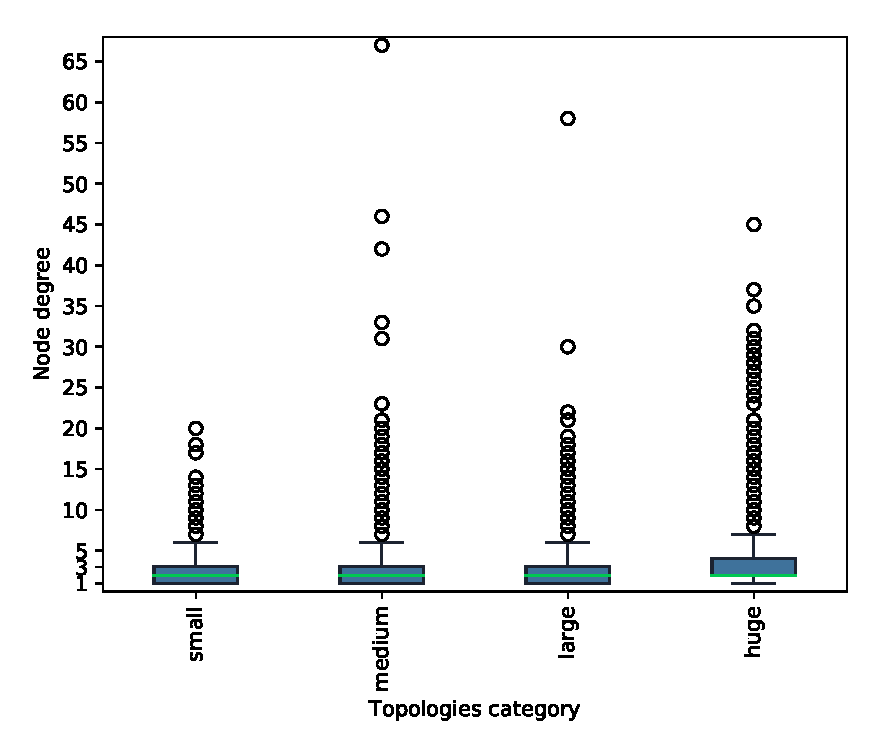
\includegraphics[width=.85\columnwidth]{./Network-lib/data/plot/deg_boxplot.eps}
\end{center}
\caption{Box plot of the degrees over the different size categories of our topologies.}
\label{fig:deg_boxplot}
\end{figure}

One degree nodes probably exist on these topologies due to the fact that most of them are were collected
using inexact methods thus leading to incomplete data. A computer network should at least be biconnected (have
at least two disjoint paths between every pair of nodes) to prevent a single link failure from partitioning
it.

The edge density of a network evaluates how close a network is from a complete graph. It is defined for graphs
with no parallel links as
$$
\frac{|E(G)|}{|V(G)| \cdot (|V(G)| - 1)}.
$$
A tree is the lowest density connected network that one can have. Any link failure in a tree will cause the network to become disconnected. High density network are costly but are more robust
to failures. They also provide a higher path diversity so optimal solution of network optimization problems tend to be
better on dense networks. Figure \ref{fig:density_cdf} shows a CDF of the densities over all topologies in
our dataset. We used the above formula even though some of our networks contain parallel links.
We can see that some network have a very low density. About $60\%$ percent of the network topologies
have an edge density of at least $10\%$ and $20\%$ of the networks have an edge density above $20\%$.

\begin{figure}
\begin{center}
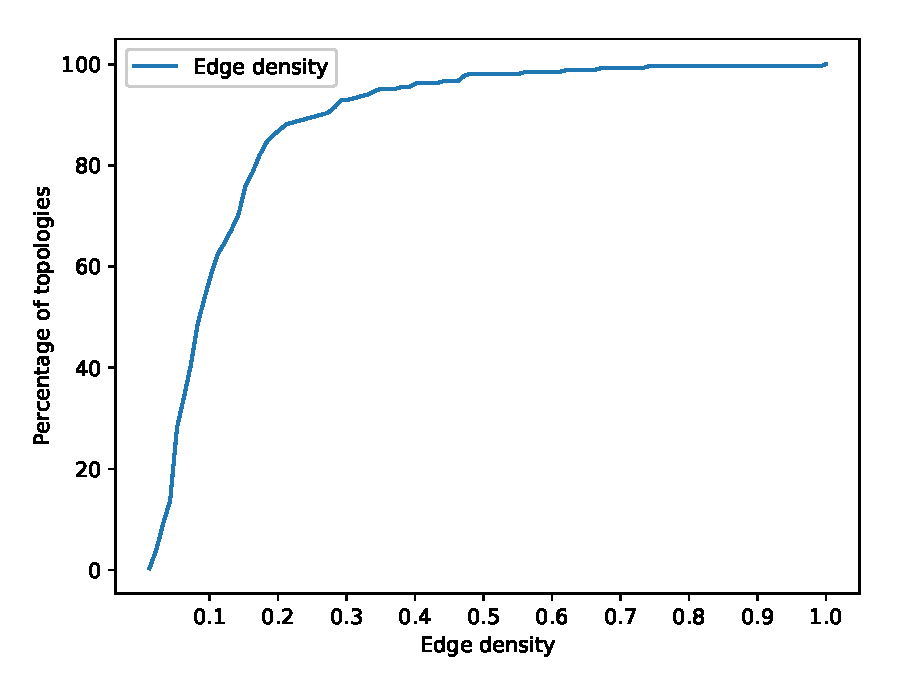
\includegraphics[width=.85\columnwidth]{./Network-lib/data/plot/edge_density.eps}
\end{center}
\caption{Box plot of the degrees over the different size categories of our topologies.}
\label{fig:density_cdf}
\end{figure}

\section{Connectivity}

We saw that some pairs of nodes have a lot of shortest paths between them. However these paths are of course not disjoint.
In this section we analyze how well the nodes are connected in the network. To measure this, we compute for each pair of nodes of each
topology the minimum number of links that need to be removed from the network in order to disconnect those nodes. This is known in graph
theory as the minimum cut between the nodes \cite{Ahuja}. Figure \ref{fig:mincut} shows a CDF of these minimum cuts. It is not hard to see
that the minimum cut between two nodes is the same as the maximum number of edge-disjoint paths between them \cite{Ahuja}.

\begin{figure}
\begin{center}
\includegraphics[width=.85\columnwidth]{./Network-lib/data/plot/minCuts.eps}
\end{center}
\caption{CDF over all topologies and all pairs of nodes of the number of shortest paths between those nodes.}
\label{fig:mincut}
\end{figure}

We can see that about $40\%$ of the pairs of nodes are connected by a single path as we had already observed above. This is quite low for a network as it does
not offer a lot of redundancy and link failures can easily disconnect the nodes. The remaining nodes require the removal of at least
$2$ links to disconnect them (in other words, they are in the same biconnected component \cite{Cormen:2009:IAT:1614191}). Also, nodes are very well connected having up to $46$ edge-disjoint paths connecting them.


\section*{Conclusion}

From this evaluation we observe that there is probably missing data on some of the topologies used in this
thesis as some of them are weakly connected. We have also seen that due to a high amout of ECMP ($26\%$) between pairs of nodes,
adjacency segments are likely to be necessary to implement paths in the graph topology with segment routing.
